\subsection{图}

例如，设 A, B, C, D, E 是五个集合，f 是从 A 到 B 的映射，g 是从 B 到 C 的映射，h 是从 D 到 E 的映射，u 是从 B 到 D 的映射，v 是从 C 到 E 的映射。为概括这样的情形，我们常使用图；例如，上述情形由下面的图概括（《集合论》第二章 §3 第 4 目）：

\begin{enumerate}
\def\labelenumi{(\arabic{enumi})}
\tightlist
\item
\end{enumerate}

\pandocbounded{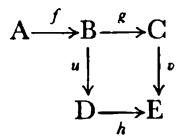
\includegraphics[keepaspectratio]{images/part001_a608eb63.jpg}}

在这样的图中，符号组 A \(\xrightarrow{f}\) B 以示意的方式表达 f 是从 A 到 B 的映射这一事实。当关于 f 不致有歧义时，我们省去字母 f 而简单地写 A \(\rightarrow\) B。

当 A, B, C, D, E 是群（相应地交换群）而 f, g, h, u, v 是群同态时，作为简称，称图 (1) 为群（相应地交换群）的图。

原则上，图不是数学对象，而只是为便于阅读论证而设计的一种图形。在实践中，图常被用作缩写符号，以避免一一列举所考虑的全部集合与映射；因此我们说“考虑图 (1)”，而不说“设 A, B, C, D, E 为五个集合……以及 v 是从 C 到 E 的映射”；例如见第 4 目中命题 2 的陈述。

